\documentclass[
    11pt,%
    aspectratio=169,%
]{beamer}

% Preamble: packages and global settings
\graphicspath{{images/}{./}}%
\usepackage{booktabs}%
\usepackage{fnpct}%
\usepackage{tikz}%
\usepackage{tabularx}
\usetikzlibrary{arrows.meta, positioning, decorations.pathreplacing, calc}

\setbeamerfont{footnote}{size=\tiny}

% Theme and colors
\usetheme{Madrid}%


\definecolor{fptBlue}{RGB}{0, 75, 145}%
\definecolor{fptOrange}{RGB}{243, 112, 33}%

% Extra colours used on the motivation slide
\definecolor{Navy}{HTML}{0B2545}%
\definecolor{LightBlue}{HTML}{E7F0FA}%
\definecolor{CardFrame}{HTML}{B9C6D6}%
\definecolor{GrayText}{HTML}{4A5568}%

% Card with picture + title + short description (motivation slide)
% #1 = image file, #2 = short title, #3 = description

\newcommand{\problemcard}[3]{%
    \begin{minipage}[t]{0.305\textwidth}
        \centering

        \includegraphics[
            width=\linewidth,
            height=1.45cm,
            keepaspectratio
        ]{#1}

        \vspace{0.05cm}

        {\color{Navy}
         \fontsize{10}{12}\selectfont
         \bfseries #2\par}

        \vspace{0.02cm}

        {\color{GrayText}
         \fontsize{8}{10}\selectfont
         \parbox{0.98\linewidth}{
             \centering #3
         }}
    \end{minipage}%
}


\setbeamercolor*{structure}{bg=fptBlue, fg=fptBlue}
\setbeamercolor*{palette primary}{use=structure, fg=white,bg=fptBlue}%
\setbeamercolor*{palette secondary}{use=structure, fg=fptBlue, bg=white}
\setbeamercolor*{palette tertiary}{use=structure, fg=white, bg=fptBlue} 

\setbeamercolor{frametitle}{bg=fptBlue, fg=white}
\setbeamercolor*{titlelike}{parent=palette primary}

    \setbeamercolor{section in head/foot}{fg=white, bg=fptOrange}
    \setbeamercolor{headline}{fg=white, bg=fptOrange}

\setbeamercolor{item projected}{bg=fptOrange}
\setbeamertemplate{enumerate items}{bg=fptOrange}

\setbeamercolor{itemize item}{fg=fptOrange}
\setbeamercolor{itemize subitem}{fg=fptOrange}

\setbeamercolor{button}{bg=fptOrange}

\setbeamercolor{section in toc}{fg=black}
\setbeamercolor{subsection in toc}{fg=black}

    \setbeamercolor{block title}{bg=fptOrange, fg=white}
    \setbeamercolor{block body}{bg=fptOrange!20}
    \setbeamercolor{block title alerted}{bg=orange, fg=white}
    \setbeamercolor{block body alerted}{bg=orange!10}
    \setbeamercolor{block title example}{bg=fptBlue, fg=white}
    \setbeamercolor{block body example}{bg=fptBlue!10}


\usepackage{graphicx}
\usepackage{array}
\usepackage{enumitem}

% Bibliography
\usepackage[backend=biber, style=numeric, sorting=none, maxbibnames=3, minbibnames=1]{biblatex}
\addbibresource{references.bib}

% Typography and slide navigation
\usefonttheme{default}%
\usepackage{palatino}%
\IfFileExists{opensans.sty}{\usepackage[default]{opensans}}{}%
\useinnertheme{circles}

\useoutertheme{miniframes}

% Presentation information
\title[NightClear]{NightClear: Joint Low-Light Image Enhancement and Deblurring}
\subtitle{A Unified Deep Learning Framework for Robust Nighttime Image Restoration}
\author[Duc, Truong, Tuan]{\texorpdfstring{%
    \begin{tabular}{ll}
        Mai Xuan Duc & SE196257 \\
        Phan Minh Nhat Truong & SE196744 \\
        Dang Thanh Tuan & SE196418
    \end{tabular}}{Mai Xuan Duc, Phan Minh Nhat Truong, Dang Thanh Tuan}}

\institute[FPTU]{Supervisor: Mr. Nguyen Trong Tai \quad$\cdot$\quad FPT University}
\date[15/11/2026]{November 15, 2026}

\newcommand{\fptlogo}{
\includegraphics[height=0.62cm]{fptu_logo.png}}
\logo{\fptlogo}


% Header and footer
\pdfstringdefDisableCommands{
    \def\translate#1{#1}
}

\setbeamerfont{section in head/foot}{size=\small, series=\bfseries}
\setbeamertemplate{headline}{}

\setbeamertemplate{sidebar right}{}
\setbeamertemplate{frametitle}{%
  \nointerlineskip
  \begin{beamercolorbox}[%
      wd=\paperwidth,
      ht=0.65cm,
      dp=0.22cm,
      leftskip=0.5cm,
      rightskip=0.5cm
  ]{frametitle}%
    \usebeamerfont{frametitle}\insertframetitle
    \hfill
    \ifnum\insertsectionnumber>1
      {\fontsize{9}{9}\selectfont\bfseries\color{white}%
       \the\numexpr\insertsectionnumber-1\relax.\enspace\insertsectionhead}%
    \fi
  \end{beamercolorbox}%
}
\setbeamertemplate{footline}{%
    \leavevmode%
    \hbox{%
        \begin{beamercolorbox}[wd=.5\paperwidth, ht=2.5ex, dp=1ex, center]{title in head/foot}%
            \usebeamerfont{title in head/foot}\inserttitle
        \end{beamercolorbox}%
        \begin{beamercolorbox}[wd=.5\paperwidth, ht=2.5ex, dp=1ex, center]{date in head/foot}%
            \usebeamerfont{date in head/foot}FPT University \quad$\cdot$\quad \insertshortdate \quad$\cdot$\quad \insertframenumber{} / \inserttotalframenumber
        \end{beamercolorbox}}%
    \vskip0pt%
}

\setbeamertemplate{navigation symbols}{}

% Slide content
\begin{document}

% 01 - Title
\section{}

\usebackgroundtemplate{%
    \begin{tikzpicture}
        \clip (0,0) rectangle (\paperwidth,\paperheight);%
        \node[inner sep=0, opacity=0.25] at ({0.5\paperwidth},{0.5\paperheight}) {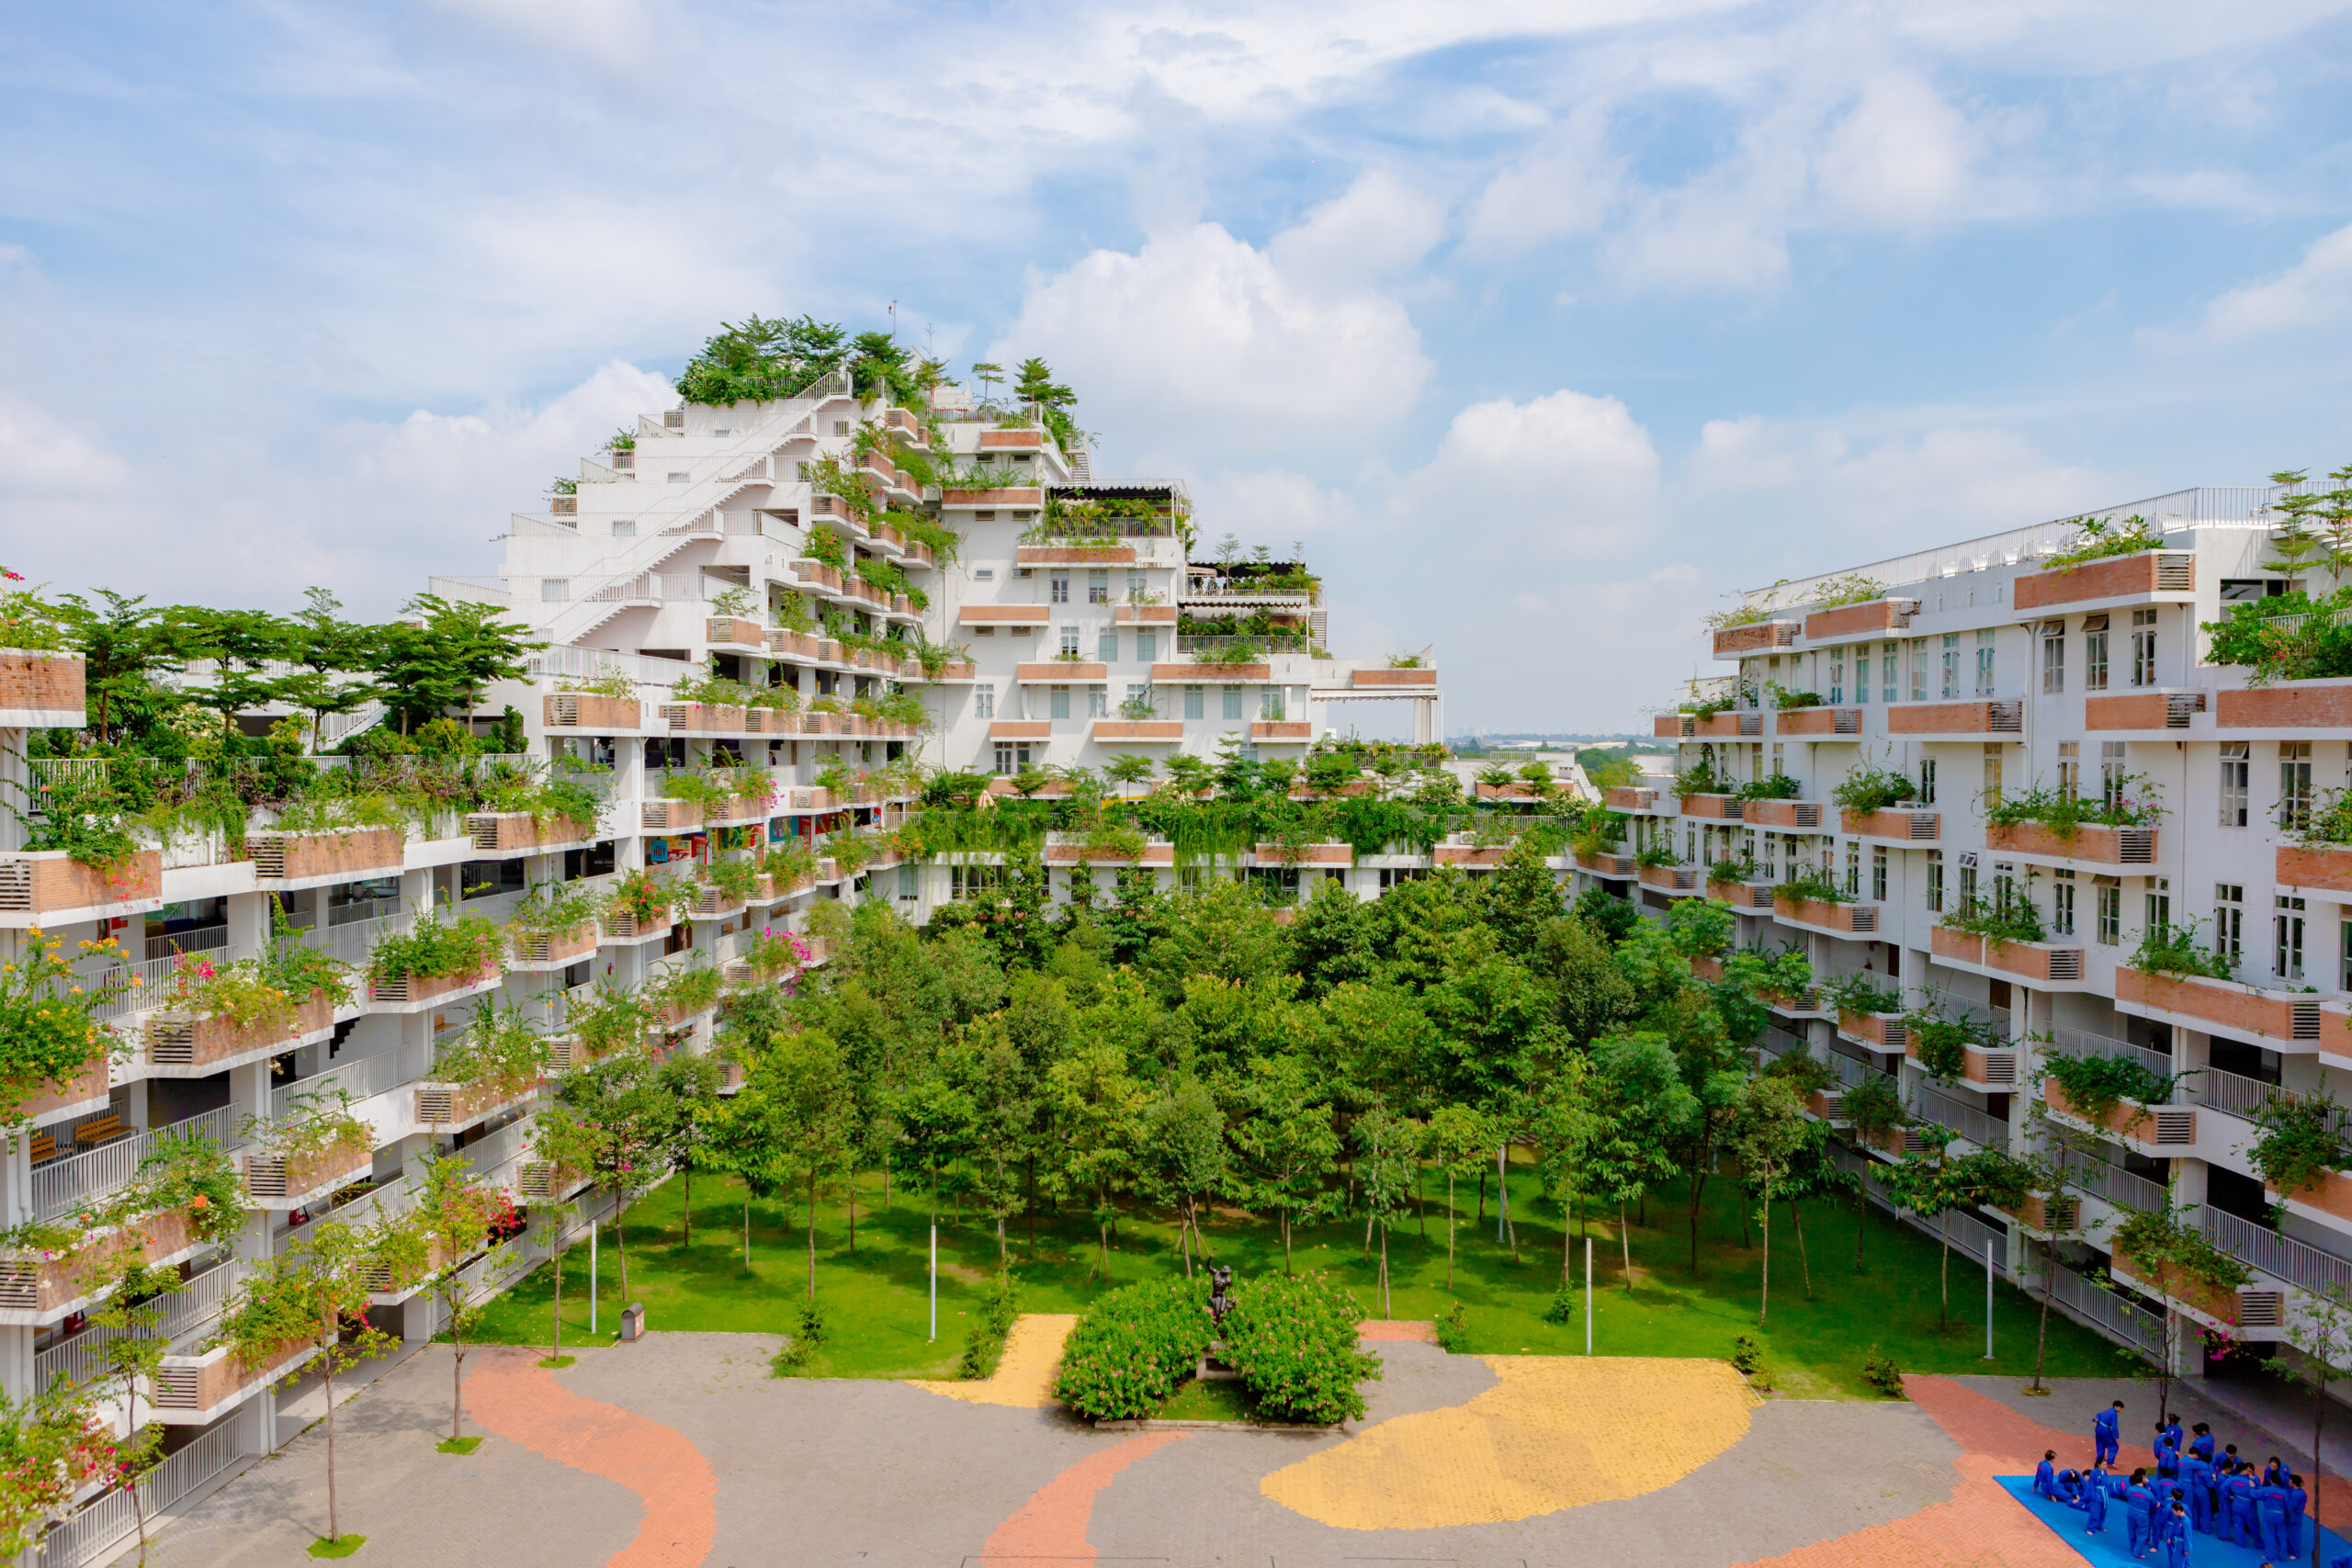
\includegraphics[width=\paperwidth]{P.Zo-9862-scaled-1.jpg}};
    \end{tikzpicture}%
}
\logo{}

\begin{frame}[plain]
    \begin{center}
        
\includegraphics[height=1.4cm]{fptu_logo.png}\\[4mm]
        \begin{beamercolorbox}[wd=0.9\textwidth, sep=9pt, center, rounded=true, shadow=true]{title}
            {\usebeamerfont{title}\inserttitle}\\[1.5mm]
            {\usebeamerfont{subtitle}\insertsubtitle}
        \end{beamercolorbox}
        \vspace{5mm}
        {\small
        \begin{tabular}{c@{\hspace{10mm}}c@{\hspace{10mm}}c}
            Mai Xuan Duc & Phan Minh Nhat Truong & Dang Thanh Tuan \\
            {\color{fptBlue}SE196257} & {\color{fptBlue}SE196744} & {\color{fptBlue}SE196418}
        \end{tabular}}\\[2.5mm]
        {\footnotesize\bfseries\color{fptOrange} SUPERVISOR}\\[0.5mm]
        {\small Mr. Nguyen Trong Tai}
        \vfill
        {\small\color{fptBlue}\bfseries Fall, 2026.}
    \end{center}
\end{frame}

\usebackgroundtemplate{}
\logo{}

% (headline removed – section shown in frametitle bar)
\setbeamercolor{title in head/foot}{fg=white, bg=fptOrange}
% (headline template is empty)


% ==========================================
% 02 - TABLE OF CONTENTS
% ==========================================
{
% Section in TOC: circle badge + right-aligned text, properly baseline-aligned
\setbeamertemplate{section in toc}{%
    \leavevmode%
    \vspace{2.5mm}%
    \noindent
    \begin{minipage}[c]{0.75cm}%
        \centering
        \tikz[baseline=-0.5ex]{%
            \node[circle, fill=orange!85, text=white,
                  minimum size=7mm, inner sep=0pt,
                  font=\fontsize{11}{11}\selectfont\bfseries]
                 {\inserttocsectionnumber};%
        }%
    \end{minipage}%
    \begin{minipage}[c]{\dimexpr\linewidth-0.80cm\relax}%
        \fontsize{14}{17}\selectfont\color{black}%
        \inserttocsection%
    \end{minipage}%
    \par%
}
}

\begin{frame}
    \frametitle{Table of Contents}

    \vspace{0.3cm}

    \begin{columns}[T,onlytextwidth]

        \begin{column}{0.48\textwidth}
            \tableofcontents[sections={2-4}]
        \end{column}

        \hfill

        \begin{column}{0.48\textwidth}
            \tableofcontents[sections={5-7}]
        \end{column}

    \end{columns}

    \vfill
\end{frame}


% ==========================================
% 03 - INTRODUCTION AND MOTIVATION
% ==========================================
\section{Introduction}

\begin{frame}{Problem Statement}

% ---------- 1. Challenges ----------
{\color{Navy}\bfseries
\fontsize{11}{13}\selectfont
Challenges in Nighttime Photography}

\vspace{0.10cm}

\begin{center}
    \problemcard
        {images/1_statement/1_1.jpg}
        {Low Illumination}
        {Insufficient light causes poor visibility
        and loss of image details.}
    \hfill
    \problemcard
        {images/1_statement/1_2.jpg}
        {Sensor Noise}
        {Low exposure increases the impact
        of sensor noise.}
    \hfill
    \problemcard
        {images/1_statement/1_3.jpg}
        {Motion Blur}
        {Camera or object motion during
        exposure causes spatial blur.}
\end{center}

\vspace{0.12cm}

% ---------- 2. Image Formation Model ----------
\begin{block}{Image Formation Model}
\vspace{0.05cm}
\begin{columns}[c,onlytextwidth]
    % Left: equation, centered vertically
    \column{0.28\textwidth}
    \centering
    $\boxed{y = \gamma(x * k) + n}$

    % Right: 2-column legend
    \column{0.72\textwidth}
    \begin{columns}[t,onlytextwidth]
        \column{0.48\textwidth}
        \begin{itemize}[leftmargin=*]
            \setlength{\itemsep}{1pt}\setlength{\parskip}{0pt}
            \item[$x$] {\small Latent sharp image.}
            \item[$k$] {\small Blur kernel (PSF).}
            \item[$*$] {\small Convolution.}
        \end{itemize}
        \column{0.52\textwidth}
        \begin{itemize}[leftmargin=*]
            \setlength{\itemsep}{1pt}\setlength{\parskip}{0pt}
            \item[$\gamma$] {\small Camera response.}
            \item[$n$]      {\small Sensor noise.}
            \item[$y$]      {\small Degraded image.}
        \end{itemize}
    \end{columns}
\end{columns}
\vspace{0.05cm}
\end{block}

\vspace{0.06cm}

\end{frame}


\begin{frame}{Project Objectives}
\small

% ---------- 1. Research Motivation ----------
\begin{beamercolorbox}[
    rounded=true,
    sep=0.06cm,
    wd=\textwidth
]{}
    \colorbox{LightBlue}{
        \parbox{\dimexpr\textwidth-2\fboxsep\relax}{
            {\color{Navy}\bfseries
            Research Motivation}

            \vspace{0.03cm}

            \fontsize{9}{11}\selectfont
            Low-light enhancement, denoising, and deblurring are
            coupled tasks; sequential processing can propagate errors,
            especially with low-quality cameras.
        }
    }
\end{beamercolorbox}

\vspace{0.18cm}

% ---------- 2. Research Objectives ----------
{\color{Navy}\bfseries Research Objectives}
\vspace{0.07cm}
\begin{columns}[T, onlytextwidth]
    % Objective 1
    \begin{column}{0.32\textwidth}
        \begin{beamercolorbox}[
            rounded=true,
            sep=0.10cm,
            wd=\linewidth
        ]{}
            {\color{orange!85!black}\bfseries 01. Low-light Enhancement}

            \vspace{0.07cm}

            \fontsize{8.5}{10}\selectfont
            Improve brightness, visibility, and natural color at night.
        \end{beamercolorbox}
    \end{column}

    % Objective 2
    \begin{column}{0.32\textwidth}
        \begin{beamercolorbox}[
            rounded=true,
            sep=0.10cm,
            wd=\linewidth
        ]{}
            {\color{orange!85!black}\bfseries 02. Quality Restoration}

            \vspace{0.07cm}

            \fontsize{8.5}{10}\selectfont
            Reduce noise and motion blur while preserving structures
            and fine detail.
        \end{beamercolorbox}
    \end{column}

    % Objective 3
    \begin{column}{0.32\textwidth}
        \begin{beamercolorbox}[
            rounded=true,
            sep=0.10cm,
            wd=\linewidth
        ]{}
            {\color{orange!85!black}\bfseries 03. Robustness and Efficiency}

            \vspace{0.07cm}

            \fontsize{8.5}{10}\selectfont
            Assess quality, speed, and robustness across camera inputs.
        \end{beamercolorbox}
    \end{column}

\end{columns}

\vspace{0.18cm}

% ---------- 3. Research Scope ----------
{\color{Navy}\bfseries Research Scope}

\vspace{0.05cm}

\begin{itemize}
    \setlength{\itemsep}{1pt}
    \setlength{\parskip}{0pt}

    \item \textbf{Reproduce:} Implement the core method and establish baselines.

    \item \textbf{Adapt:} Test on low-resolution, noisy images from low-quality cameras.

    \item \textbf{Extend:} Explore evidence-based gains in robustness and efficiency.
\end{itemize}

\end{frame}


% 04 - Related Work
\section{Related Work}

\begin{frame}{Existing Approaches}
\small
% ---------- 1. Literature Overview ----------
{\color{Navy}\bfseries
Representative Image Restoration Methods}

\vspace{0.12cm}

\renewcommand{\arraystretch}{1.5}

\begin{tabularx}{\textwidth}{
    >{\raggedright\arraybackslash}p{0.24\textwidth}
    >{\raggedright\arraybackslash}p{0.38\textwidth}
    >{\raggedright\arraybackslash}X
}

\toprule

\textbf{\color{Navy}Approach} &
\textbf{\color{Navy}Representative Methods} &
\textbf{\color{Navy}Primary Objective} \\

\midrule

\textbf{Low-light Enhancement} & RetinexNet \cite{wei2018retinexnet}, Zero-DCE \cite{guo2020zerodce} & Illumination and contrast enhancement \\
\textbf{Image Deblurring} & DeblurGAN \cite{kupyn2018deblurgan}, NAFNet \cite{chen2022nafnet} & Blur removal and detail restoration \\
\textbf{Joint Restoration} & LEDNet \cite{zhou2022lednet}, DarkIR \cite{feijoo2025darkir} & Joint low-light enhancement and deblurring / multi-task restoration \\
\bottomrule
\end{tabularx}
\vspace{0.3cm}
\end{frame} 

\begin{frame}{Existing Approaches}
\small
% ---------- 2. Limitation ----------
{\color{Navy}\bfseries
Limitation of Sequential Restoration}

\vspace{0.22cm}

\begin{center}


\begin{tikzpicture}[
    node distance=0.65cm,
    process/.style={
        draw=Navy!65,
        fill=LightBlue!45,
        rounded corners=3pt,
        minimum width=2.55cm,
        minimum height=0.72cm,
        align=center,
        font=\small\bfseries,
        text=Navy
    },
    annotation/.style={
        font=\scriptsize,
        text=orange!85!black,
        align=center
    },
    arrow/.style={
        -{Stealth[length=2.2mm]},
        thick,
        draw=Navy!75
    }
]

\node[process] (input)
{Low-light Input};

\node[process, right=of input] (enhance)
{Enhancement};

\node[process, right=of enhance] (deblur)
{Deblurring};

\node[process, right=of deblur] (output)
{Restored Image};

\draw[arrow] (input) -- (enhance);
\draw[arrow] (enhance) -- (deblur);
\draw[arrow] (deblur) -- (output);

\node[annotation, below=0.13cm of enhance]
{Noise amplification \cite{wei2018retinexnet}};

\node[annotation, below=0.13cm of deblur]
{Error propagation \cite{zhou2022lednet}};

\end{tikzpicture}

\end{center}

\vspace{0.12cm}

\begin{itemize}
    \setlength{\itemsep}{2pt}
    \item Enhancement may amplify existing noise in low-light images.
    \item Cascaded enhancement and deblurring may not effectively handle coupled visibility and sharpness degradation. \cite{zhou2022lednet}
\end{itemize}

\vspace{0.12cm}

% ---------- 3. Research Motivation ----------

\begin{beamercolorbox}[
    rounded=true,
    sep=0.08cm,
    wd=\textwidth
]{}

\colorbox{LightBlue}{
    \parbox{\dimexpr\textwidth-2\fboxsep\relax}{
        {\color{Navy}\bfseries
        Research Motivation}

        \vspace{0.05cm}

        \fontsize{9}{11}\selectfont

        Joint restoration provides a unified approach
        to addressing multiple image degradations,
        motivating the investigation of robust
        nighttime image restoration under challenging
        imaging conditions \cite{zhou2022lednet,feijoo2025darkir}.
    }
}

\end{beamercolorbox}
\end{frame}


\begin{frame}
    \frametitle{Key EDA Insights (1/2): How Dark Is the Data?}
    \framesubtitle{LOLv2 real + synthetic, all 1{,}789 pairs, luminance $Y \in [0, 1]$}

    \begin{center}
        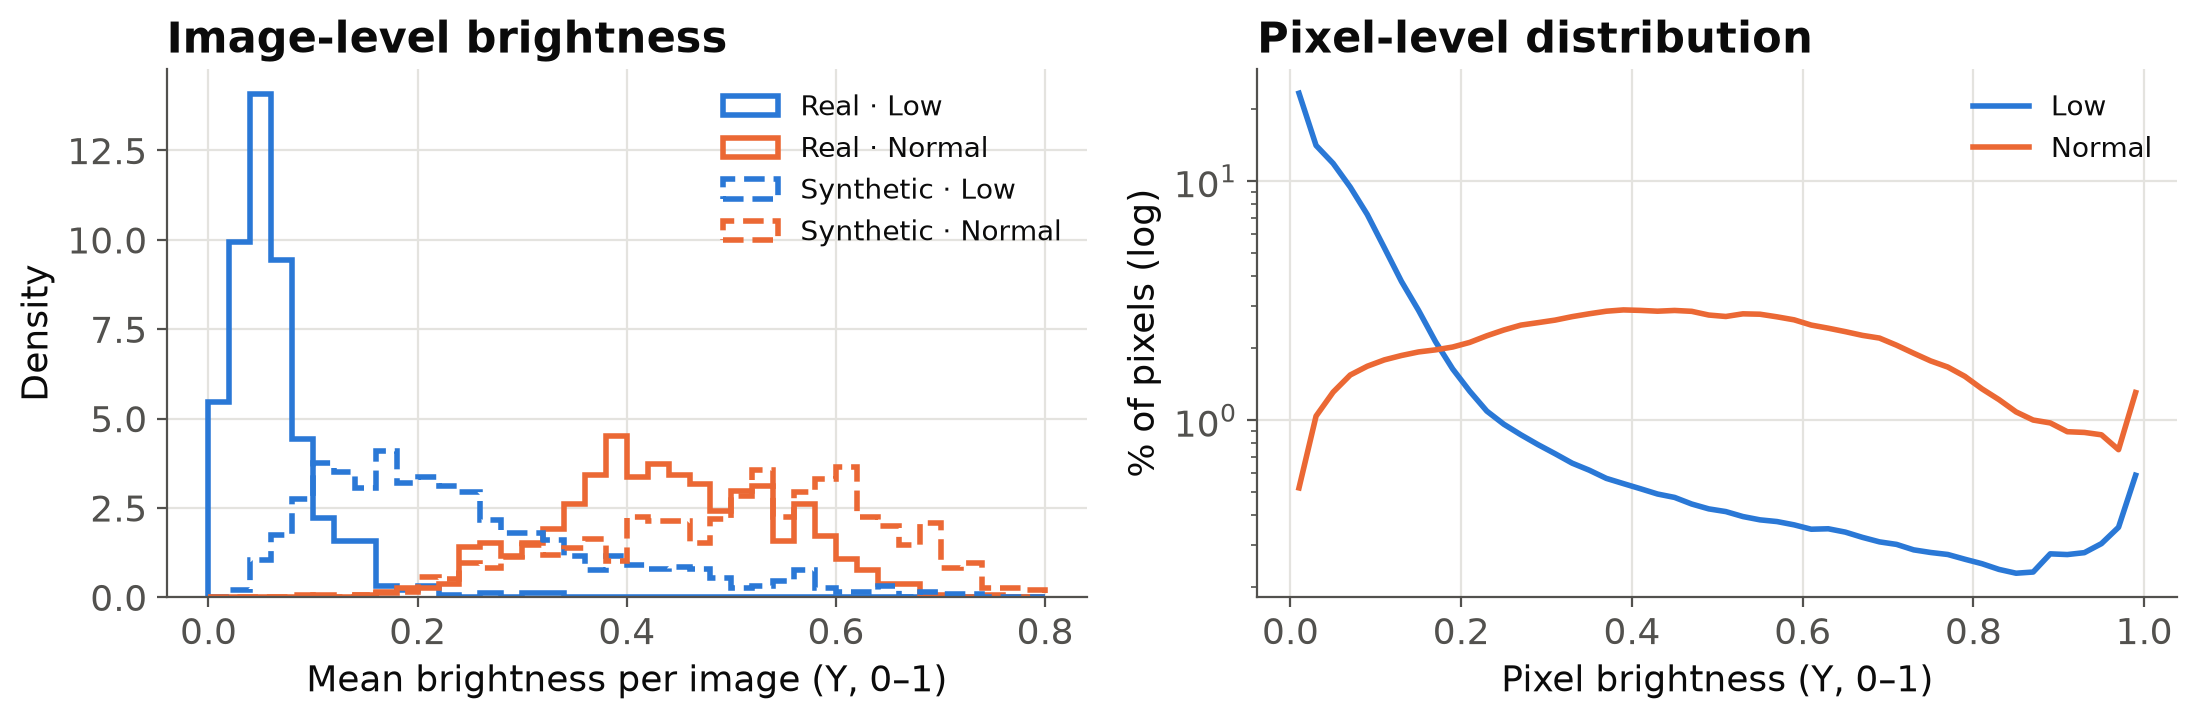
\includegraphics[width=\textwidth, height=0.52\textheight, keepaspectratio]{eda/brightness.png}
    \end{center}
    \vspace{-2mm}
    \begin{columns}[t]
        \begin{column}{0.5\textwidth}
            \footnotesize
            \textbf{Left:} real low-light images average $Y = 0.06$ vs.\ $0.44$ for GT; synthetic ones are much brighter ($0.24$) $\Rightarrow$ \textbf{real/synthetic domain gap}.
        \end{column}
        \begin{column}{0.5\textwidth}
            \footnotesize
            \textbf{Right:} 81\% of real low-light pixels have $Y < 0.1$ $\Rightarrow$ most information sits in a few dark grey levels, where noise dominates.
        \end{column}
    \end{columns}
\end{frame}

\begin{frame}
    \frametitle{Key EDA Insights (2/2): Brightening Is Not One Curve}
    \begin{columns}[c]
        \begin{column}{0.5\textwidth}
            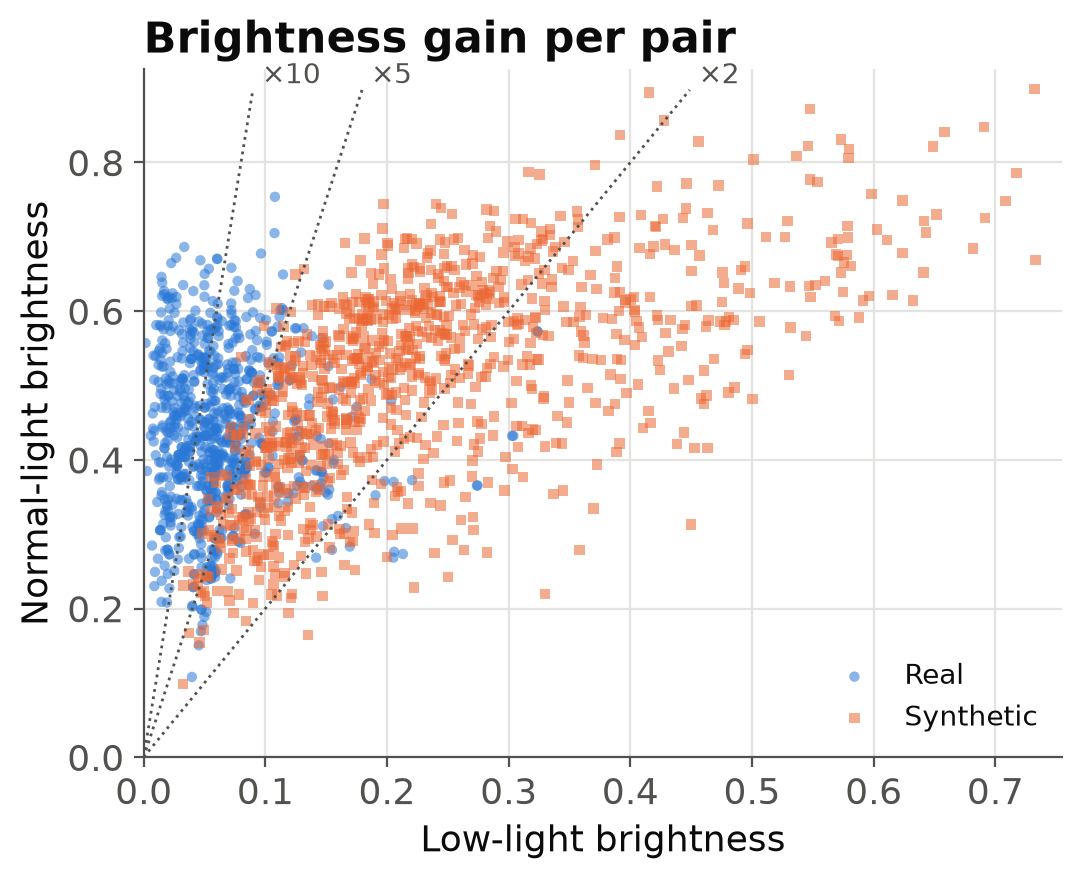
\includegraphics[width=\textwidth]{eda/gain_scatter.png}
        \end{column}
        \begin{column}{0.48\textwidth}
            \small
            Gain = GT brightness / low-light brightness
            \begin{itemize}
                \item Real: median $\times 7.5$, 90\% of pairs between $\times 2.8$ and $\times 30$.
                \item Synthetic: median $\times 2.5$ ($\times 1.1$ -- $\times 4.8$).
            \end{itemize}
            \vspace{2mm}
            \textbf{Conclusion:} the required brightening changes from image to image, so a global curve (gamma, histogram equalisation) cannot fit all pairs $\Rightarrow$ the model must learn \emph{content-aware} enhancement.
        \end{column}
    \end{columns}
\end{frame}
% 05 - Methodology and architecture
\section{Method}

\begin{frame}
    \frametitle{Solution Pipeline}
    \framesubtitle{Train once on paired images, then restore new photos on the local machine}

    \centering
    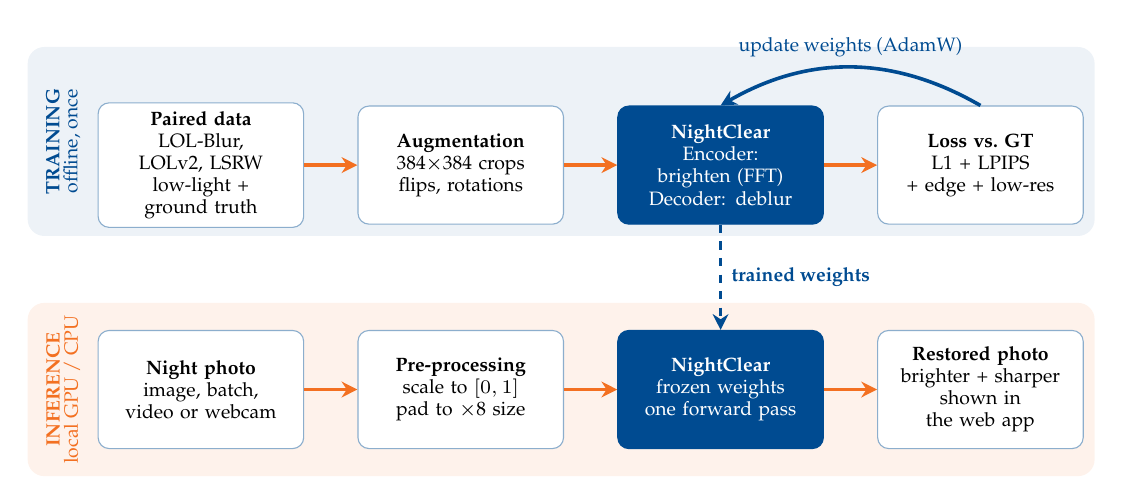
\begin{tikzpicture}[
        box/.style={rounded corners=4pt, draw=fptBlue!45, fill=white, text width=2.4cm, align=center,
                    minimum height=1.5cm, font=\scriptsize, inner sep=3pt},
        net/.style={box, fill=fptBlue, draw=fptBlue, text=white},
        flow/.style={-{Stealth[length=2mm, width=2mm]}, line width=1.3pt, fptOrange},
        lane/.style={rounded corners=6pt, draw=none},
        lanelabel/.style={rotate=90, font=\scriptsize\bfseries, align=center}]

        \fill[lane, fptBlue!7]   (-2.2,-0.9) rectangle (11.35,1.5);
        \fill[lane, fptOrange!9] (-2.2,-3.95) rectangle (11.35,-1.75);
        \node[lanelabel, text=fptBlue]   at (-1.75,0.3)  {TRAINING\\[-0.5mm]\mdseries offline, once};
        \node[lanelabel, text=fptOrange] at (-1.75,-2.85) {INFERENCE\\[-0.5mm]\mdseries local GPU / CPU};

        \node[box] (d)  at (0,0)   {\textbf{Paired data}\\ LOL-Blur, LOLv2, LSRW\\ low-light + ground truth};
        \node[box] (a)  at (3.3,0) {\textbf{Augmentation}\\ 384$\times$384 crops\\ flips, rotations};
        \node[net] (m)  at (6.6,0) {\textbf{NightClear}\\ Encoder: brighten (FFT)\\ Decoder: deblur};
        \node[box] (l)  at (9.9,0) {\textbf{Loss vs.\ GT}\\ L1 + LPIPS\\ + edge + low-res};
        \draw[flow] (d) -- (a);
        \draw[flow] (a) -- (m);
        \draw[flow] (m) -- (l);
        \draw[flow, fptBlue] (l.north) to[out=150, in=30]
            node[above, font=\scriptsize, text=fptBlue] {update weights (AdamW)} (m.north);

        \node[box] (i)  at (0,-2.85)   {\textbf{Night photo}\\ image, batch,\\ video or webcam};
        \node[box] (p)  at (3.3,-2.85) {\textbf{Pre-processing}\\ scale to $[0,1]$\\ pad to $\times$8 size};
        \node[net] (m2) at (6.6,-2.85) {\textbf{NightClear}\\ frozen weights\\ one forward pass};
        \node[box] (o)  at (9.9,-2.85) {\textbf{Restored photo}\\ brighter + sharper\\ shown in the web app};
        \draw[flow] (i) -- (p);
        \draw[flow] (p) -- (m2);
        \draw[flow] (m2) -- (o);

        \draw[flow, fptBlue, dashed] (m.south) -- node[right, font=\scriptsize\bfseries, text=fptBlue] {trained weights} (m2.north);
    \end{tikzpicture}
\end{frame}

\begin{frame}
    \frametitle{NightClear Architecture \& Training}

    \begin{center}
        \includegraphics[height=0.37\textheight]{../../assets/networks-scheme.png}
    \end{center}
    \vspace{-1mm}
    \begin{columns}[t]
        \begin{column}{0.5\textwidth}
            \footnotesize
            \textbf{Encoder = illumination (Fourier domain)}
            \begin{itemize}
                \item EBlock: attention + \textbf{FreMLP} (MLP on the FFT \emph{amplitude})
                \item Bottleneck predicts an 8$\times$ smaller lit image
            \end{itemize}
            \textbf{Decoder = deblurring (spatial domain)}
            \begin{itemize}
                \item DBlock: \textbf{Di-SpAM}, dilated depthwise convs (1, 4, 9)
            \end{itemize}
        \end{column}
        \begin{column}{0.5\textwidth}
            \footnotesize
            \textbf{Training}
            \begin{itemize}
                \item Loss: $\mathcal{L} = \mathcal{L}_{1} + 0.01\,\mathcal{L}_{\text{LPIPS}} + 50\,\mathcal{L}_{\text{edge}} + \mathcal{L}_{\text{low-res}}$
                \item AdamW, LR $5\!\times\!10^{-4} \rightarrow 10^{-6}$ cosine, batch 32, H100
                \item NightClear-m: width 32, \textbf{3.31 M params, 7.25 GMACs}
            \end{itemize}
        \end{column}
    \end{columns}
\end{frame}
% 06 - Results and evaluation
\section{Results}

\begin{frame}
    \frametitle{Model Experimentation}
    \framesubtitle{Baselines vs.\ advanced models on LOLBlur}

    \begin{columns}[t]
        \begin{column}{0.56\textwidth}
            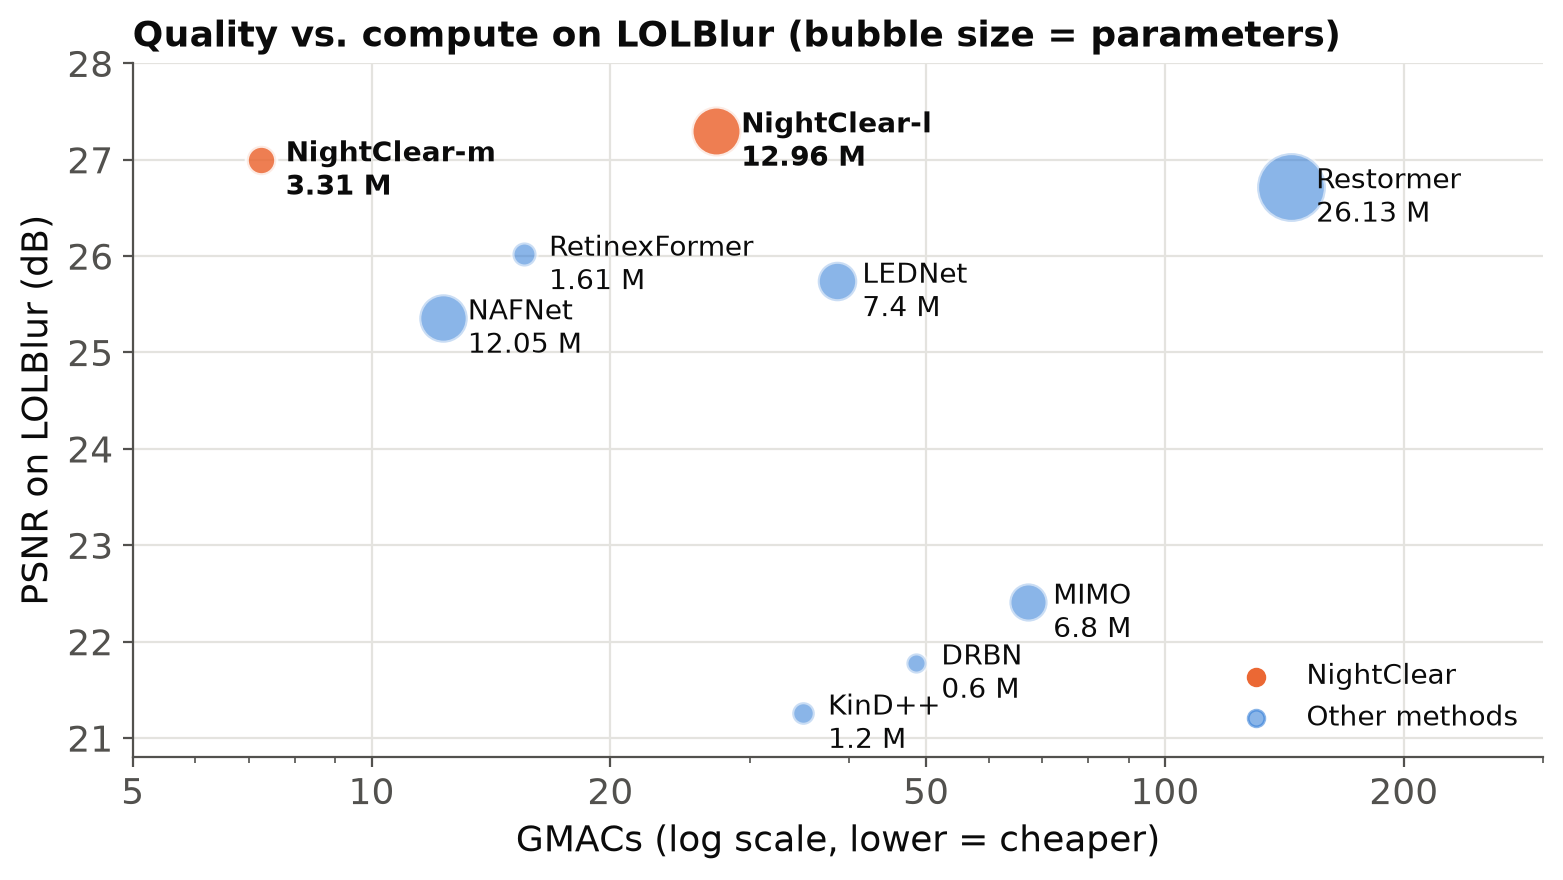
\includegraphics[width=\textwidth, height=0.55\textheight, keepaspectratio]{results/efficiency.png}\\
            \footnotesize NightClear-m reaches the best PSNR with the \textbf{lowest compute} (7.25 GMACs, 20$\times$ less than Restormer).
        \end{column}
        \begin{column}{0.42\textwidth}
            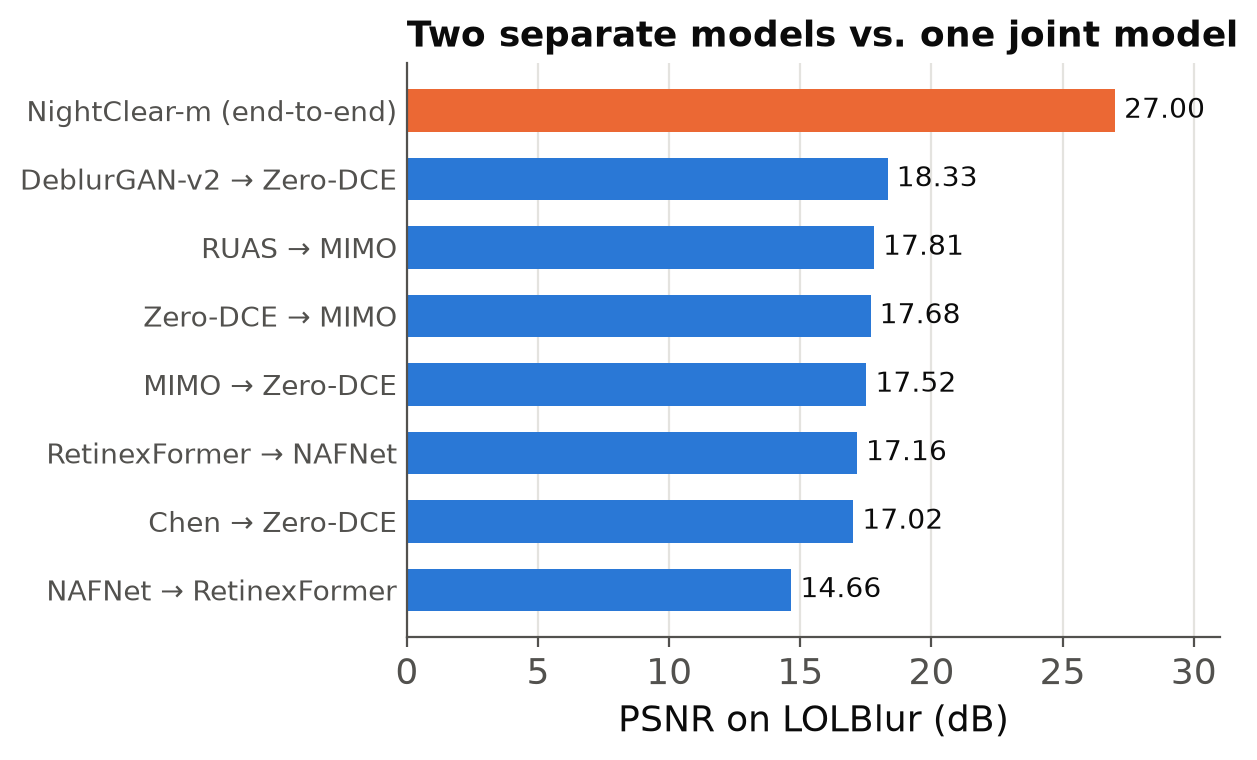
\includegraphics[width=\textwidth, height=0.55\textheight, keepaspectratio]{results/cascade.png}\\
            \footnotesize Every two-model cascade stays below 18.4\,dB; one joint model gains \textbf{+8.7\,dB}.
        \end{column}
    \end{columns}
    \vspace{1mm}
    {\tiny DeblurGAN-v2 (22.30 dB) is not plotted: no MACs available.}
\end{frame}

\begin{frame}
    \frametitle{Evaluation Across Datasets}
    \framesubtitle{Best other method per row; bold = better value}

    \begin{center}
    \footnotesize
    \setlength{\tabcolsep}{4.5pt}
    \begin{tabular}{lllll}
        \toprule
        \textbf{Dataset} & \textbf{Metric} & \textbf{NightClear} & \textbf{Best other method} & \\
        \midrule
        LOLBlur & PSNR $\uparrow$  & \textbf{27.00} (m) / \textbf{27.30} (l) & 26.72 & Restormer \\
                & SSIM $\uparrow$  & 0.883 / 0.898 & \textbf{0.902} & Restormer \\
                & LPIPS $\downarrow$ & 0.162 / 0.137 & \textbf{0.133} & Restormer \\
        LOLv2-real  & PSNR / SSIM & \textbf{23.87} / \textbf{0.880} & 22.80 / 0.840 & Retinexformer \\
        LOLv2-synth & PSNR / SSIM & 25.54 / \textbf{0.934} & \textbf{25.67} / 0.930 & Retinexformer \\
        LSRW        & PSNR / SSIM & \textbf{18.93} / \textbf{0.583} & 17.67 / 0.549 & FIDE \\
        Real-LOLBlur & MUSIQ $\uparrow$ / NIQE $\downarrow$ & 48.36 / 4.998 & \textbf{50.22} / \textbf{4.576} & NAFNet / Retinexformer \\
        \bottomrule
    \end{tabular}
    \end{center}
    \vspace{1mm}
    \footnotesize
    \begin{itemize}
        \item Best PSNR on 3 of the 4 paired benchmarks, with 8$\times$ fewer parameters than Restormer.
        \item Not the best everywhere: Restormer has better SSIM / LPIPS on LOLBlur, and on real blurry night photos (no GT) NightClear is competitive but not first.
    \end{itemize}
    {\tiny LOLv2 / LSRW use NightClear-mt (multi-task model, 26.62 dB on LOLBlur).}
\end{frame}

\begin{frame}
    \frametitle{Error Analysis}
    \framesubtitle{Released outputs on LOLv2-real image 00733: where does each model fail?}

    \begin{center}
        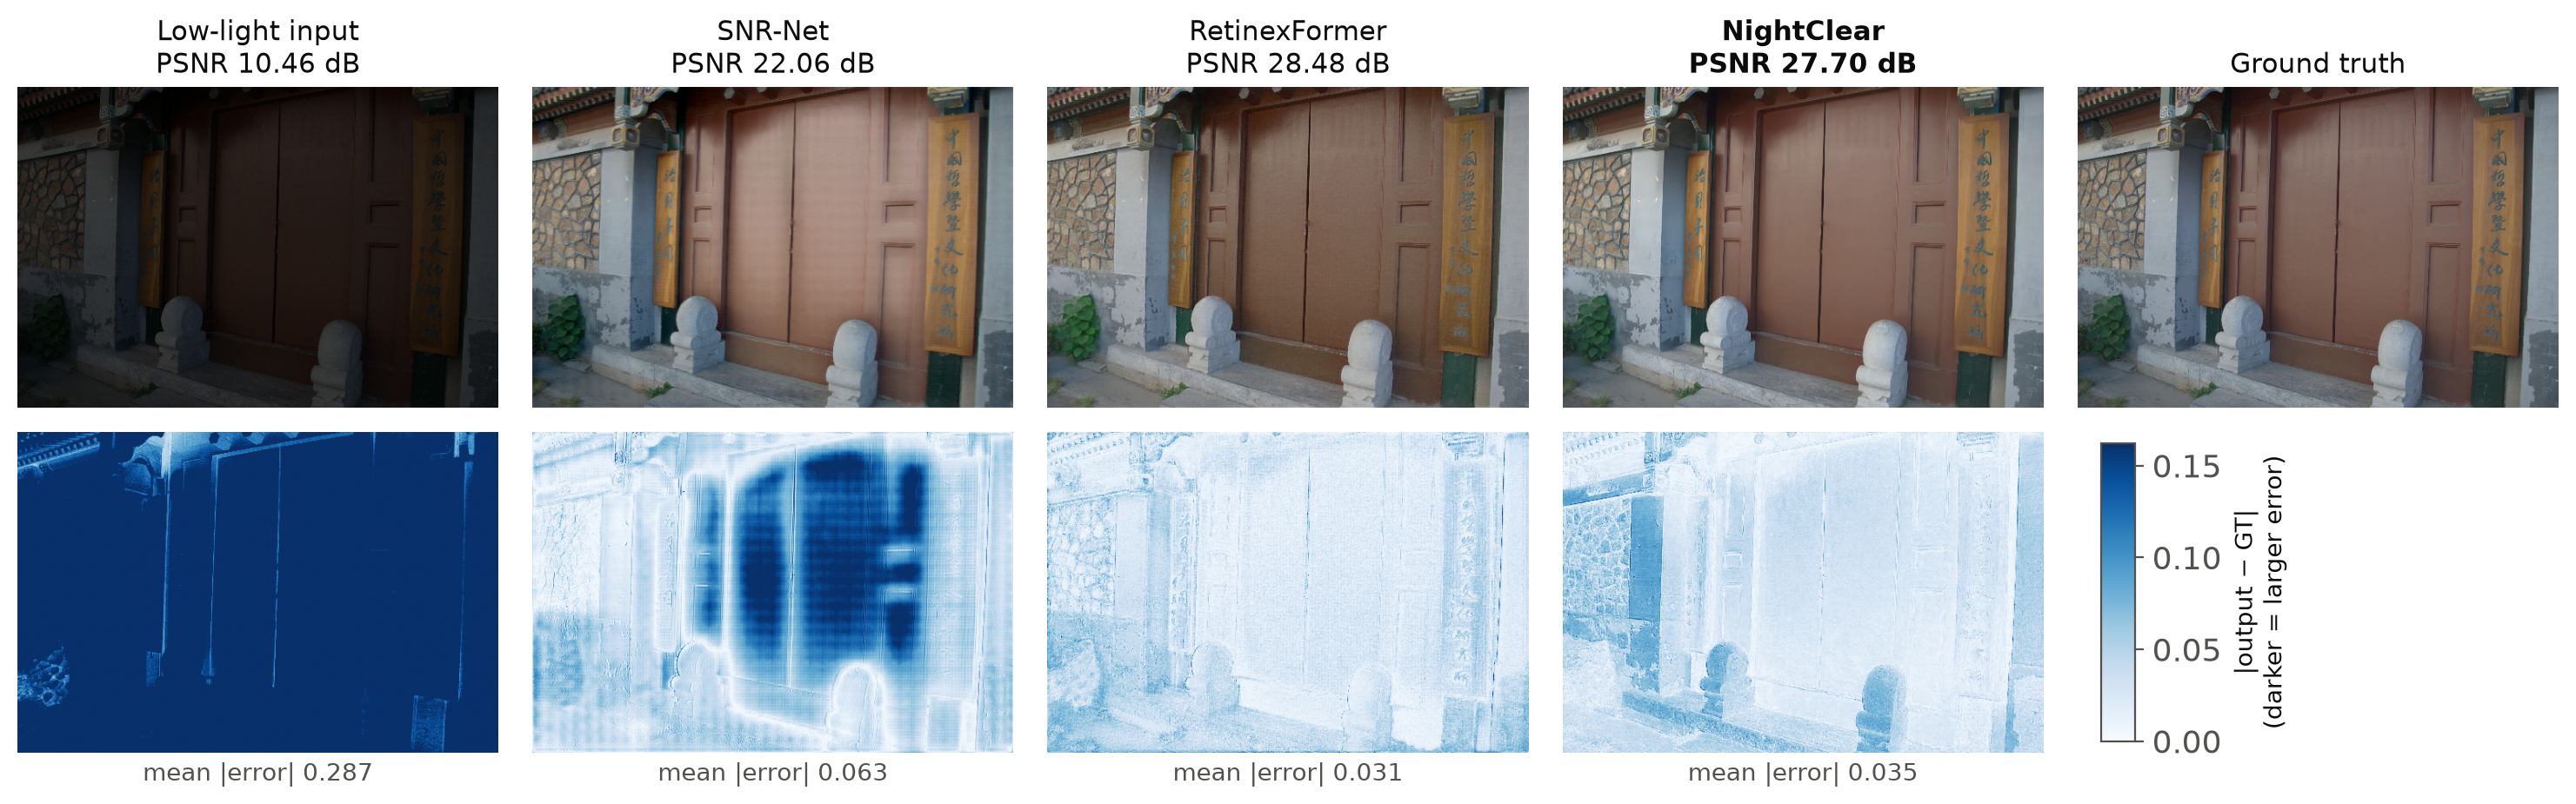
\includegraphics[width=\textwidth, height=0.46\textheight, keepaspectratio]{results/error_maps.png}
    \end{center}
    \footnotesize
    \begin{itemize}
        \item On this image Retinexformer (28.48\,dB) beats NightClear (27.70\,dB): NightClear's errors sit on the \textbf{textured stone wall and dark shadows} (tone shift).
        \item SNR-Net leaves blotchy artefacts on the large flat door.
        \item Takeaway: what remains is mostly \textbf{tone error in dark, textured regions}, consistent with the EDA (very dark pixels carry little signal).
    \end{itemize}
\end{frame}
% 07 - Model interpretability
\begin{frame}
    \frametitle{Model Interpretability (1/2): Which Components Matter?}
    \framesubtitle{Component importance = PSNR lost when a part is removed or replaced}

    \begin{center}
        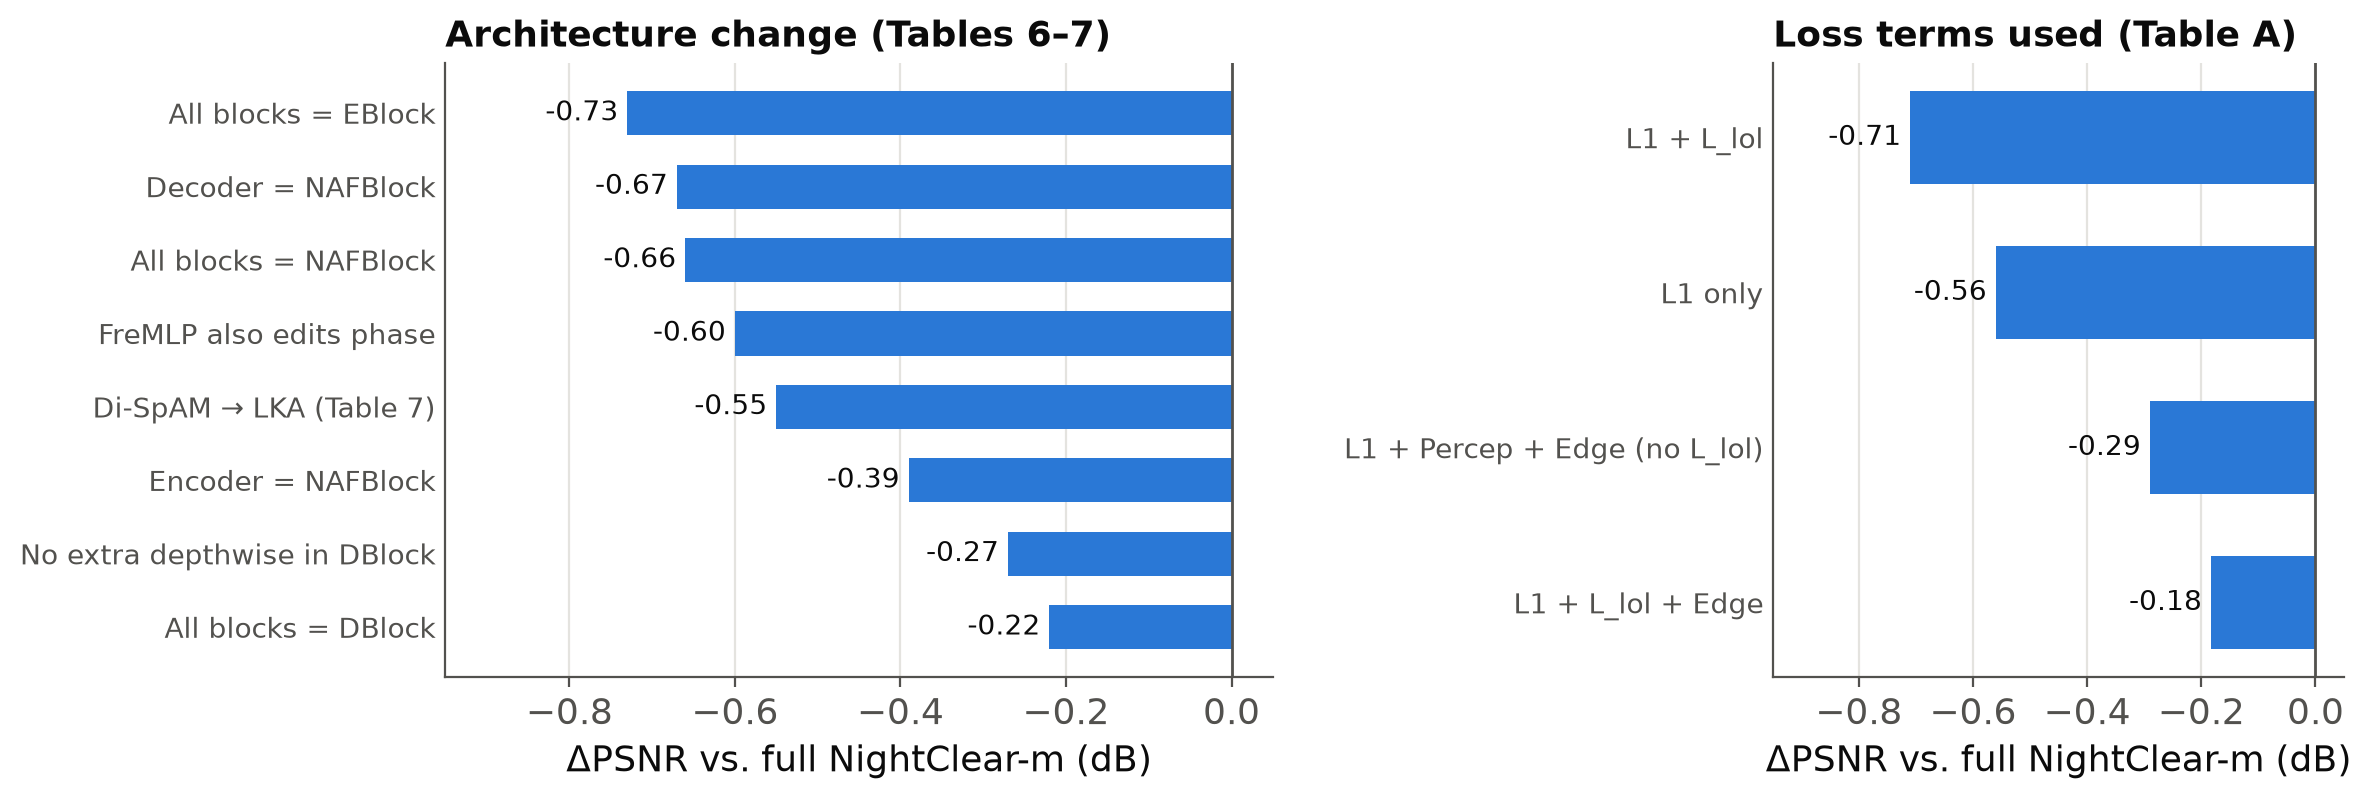
\includegraphics[width=\textwidth, height=0.47\textheight, keepaspectratio]{results/ablation.png}
    \end{center}
    \footnotesize
    \begin{itemize}
        \item Using the \textbf{same block everywhere} costs up to 0.73\,dB: the encoder (illumination) and the decoder (deblurring) need different designs.
        \item The low-res supervision $\mathcal{L}_{\text{low-res}}$ only helps together with the perceptual and edge losses (all four terms give the best PSNR).
    \end{itemize}
    {\tiny Ablations trained on 256\,px crops (full model 26.90\,dB); Di-SpAM $\rightarrow$ LKA row vs.\ 27.00\,dB.}
\end{frame}

\begin{frame}
    \frametitle{Model Interpretability (2/2): Why the Fourier Amplitude?}
    \framesubtitle{Our experiment on the 100 LOLv2-real test pairs: swap the FFT amplitude, keep the phase}

    \begin{center}
        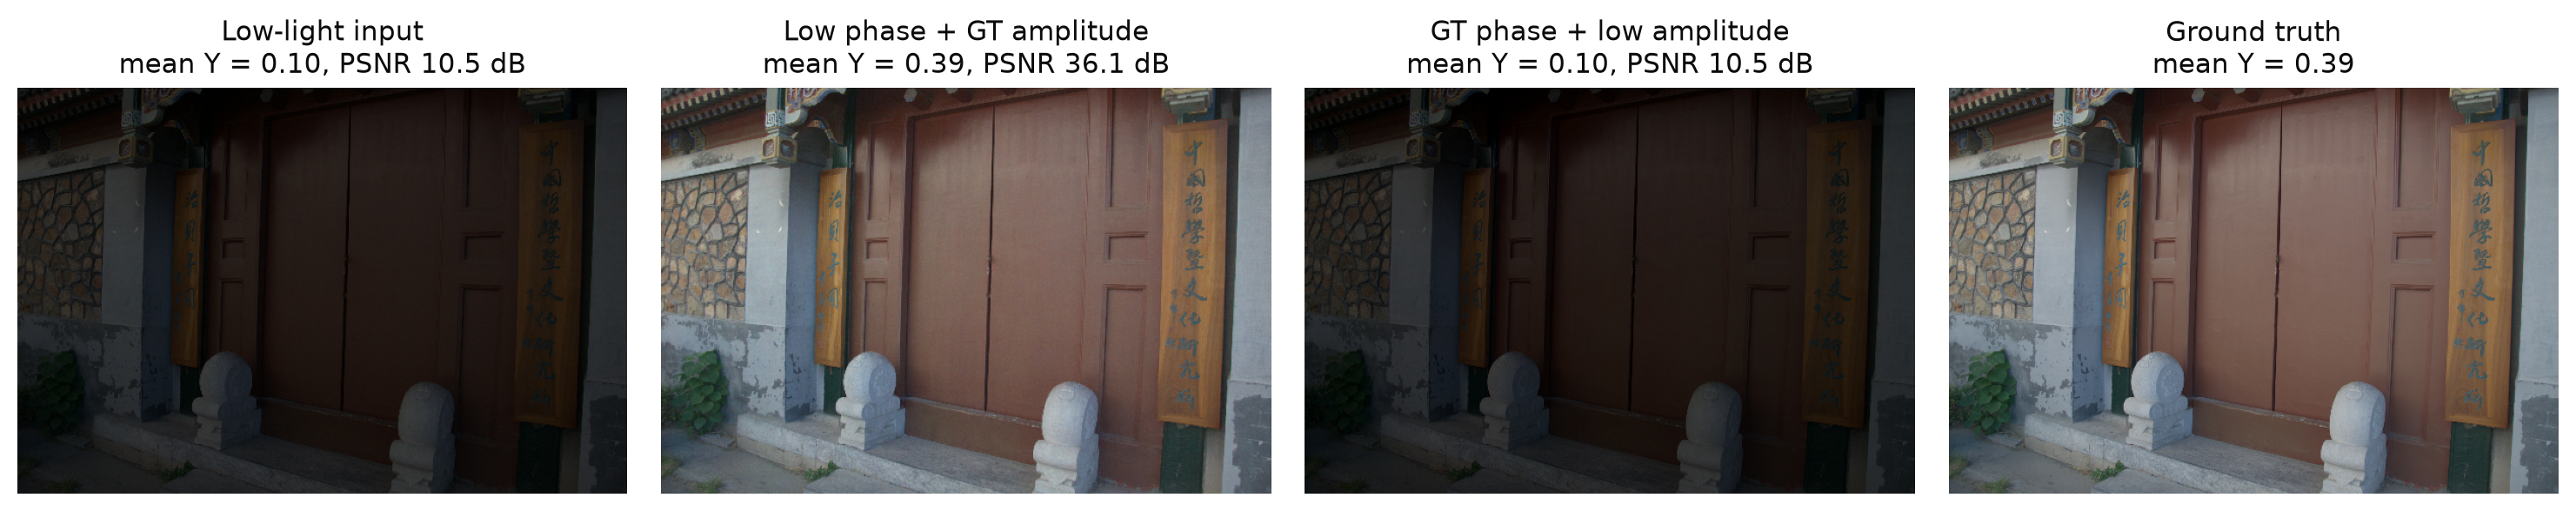
\includegraphics[width=\textwidth, height=0.36\textheight, keepaspectratio]{results/amplitude_swap.png}
    \end{center}
    \begin{columns}[t]
        \begin{column}{0.55\textwidth}
            \footnotesize
            \begin{itemize}
                \item Low-light \textbf{phase} + GT \textbf{amplitude} $\approx$ the GT image: mean PSNR \textbf{9.72 $\rightarrow$ 29.07\,dB} over 100 pairs.
                \item GT phase + low amplitude stays dark: brightness lives in the amplitude, structure in the phase.
            \end{itemize}
        \end{column}
        \begin{column}{0.43\textwidth}
            \footnotesize
            $\Rightarrow$ This explains the design: \textbf{FreMLP} edits only the amplitude, and letting it change the phase too \textbf{lowers PSNR by 0.60\,dB}.
        \end{column}
    \end{columns}
\end{frame}
% 08 - Product demo and practical impact
\section{Demo}

\begin{frame}
    \frametitle{Product Demo: NightClear Web App}
    \framesubtitle{Web application built with Gradio}

    \begin{columns}[c]
        \begin{column}{0.62\textwidth}
            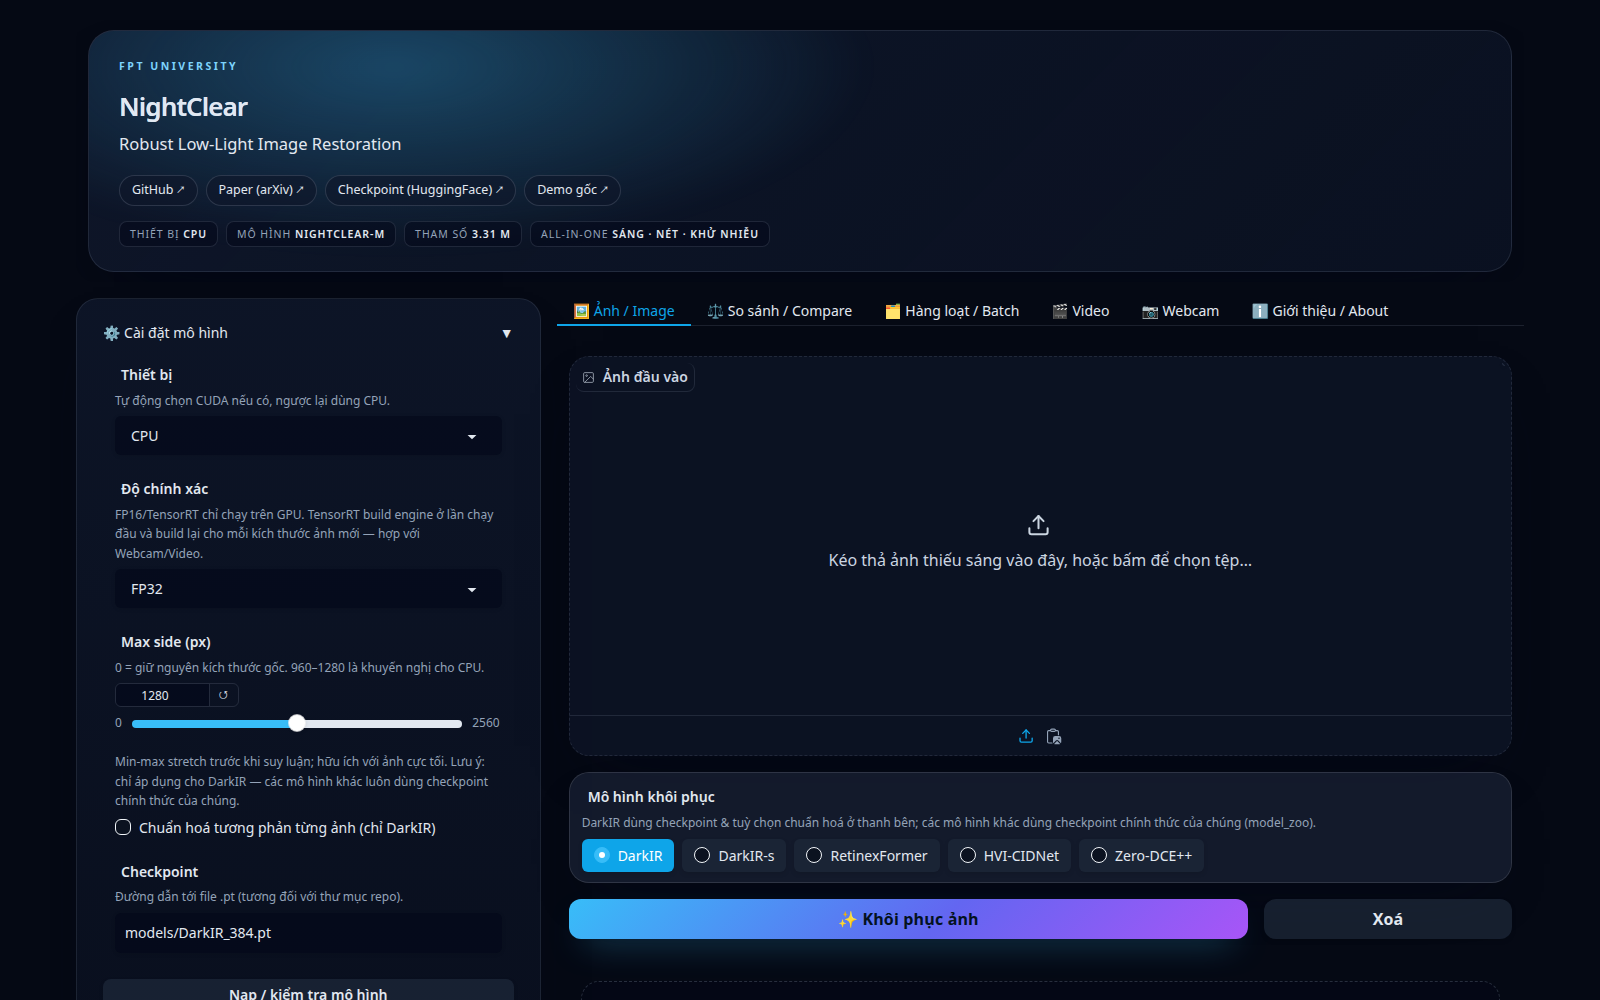
\includegraphics[width=\textwidth]{demo/ui.png}
        \end{column}
        \begin{column}{0.37\textwidth}
            \footnotesize
            \begin{itemize}
                \item \textbf{Tabs}: Image, Compare, Batch, Video, Webcam
                \item \textbf{5 models}: NightClear, NightClear-s, RetinexFormer, HVI-CIDNet, Zero-DCE++
                \item \textbf{Compare}: all models on one photo, ranked by speed
                \item \textbf{Precision}: FP32, FP16, TensorRT
                \item Runs on the local GPU or on CPU
            \end{itemize}
        \end{column}
    \end{columns}
\end{frame}

\newcommand{\stat}[2]{%
    \begin{beamercolorbox}[wd=\linewidth, ht=1.6cm, dp=0pt, center, rounded=true]{block body example}
        {\LARGE\bfseries\color{fptOrange} #1}\\[1mm]{\scriptsize #2}
    \end{beamercolorbox}}

\begin{frame}
    \frametitle{Practical Impact}

    \begin{columns}[t]
        \begin{column}{0.24\textwidth}\stat{+8.7 dB}{vs.\ best 2-model cascade}\end{column}
        \begin{column}{0.24\textwidth}\stat{5.3$\times$}{fewer MACs than LEDNet}\end{column}
        \begin{column}{0.24\textwidth}\stat{$-$55\%}{parameters vs.\ LEDNet}\end{column}
        \begin{column}{0.24\textwidth}\stat{3.31 M}{params, 13 MB, runs on CPU}\end{column}
    \end{columns}
    \vspace{2mm}
    \begin{columns}[t]
        \begin{column}{0.5\textwidth}
            \small
            \textbf{Value}
            \begin{itemize}
                \item One network instead of two to store, tune and run
                \item Fits laptops and a single local GPU
                \item Handheld night shots without tripod or flash
            \end{itemize}
        \end{column}
        \begin{column}{0.5\textwidth}
            \small
            \textbf{Applications}
            \begin{itemize}
                \item Smartphone night mode
                \item Night surveillance / dash cams
                \item Pre-processing for detection in the dark (e.g.\ ExDark)
            \end{itemize}
        \end{column}
    \end{columns}
    {\tiny Runtime is not benchmarked yet, so no time saving is claimed.}
\end{frame}
% 09 - Limitations, future work, and conclusion
\section{Conclusion}

\begin{frame}
    \frametitle{Limitations \& Future Work}
    \begin{columns}[t]
        \begin{column}{0.5\textwidth}
            \footnotesize
            \textbf{Limitations}
            \begin{itemize}
                \item Depthwise convs: few MACs but not GPU-friendly, so speed gains are smaller than compute gains
                \item No runtime benchmark yet (only MACs / parameters)
                \item Not best on every metric (SSIM/LPIPS on LOLBlur, real photos)
                \item Real/synthetic gap in the data (EDA)
                \item Our app: TensorRT disabled for RetinexFormer / HVI-CIDNet (wrong outputs); NightClear-s weights not bundled
            \end{itemize}
        \end{column}
        \begin{column}{0.5\textwidth}
            \footnotesize
            \textbf{Future work}
            \begin{itemize}
                \item Measure latency on phone / edge GPUs; INT8 quantisation
                \item Video: temporal consistency between frames
                \item Collect real paired night data (e.g.\ with a tripod) to close the domain gap
                \item Train jointly with a detector for night-time object detection
            \end{itemize}
        \end{column}
    \end{columns}
\end{frame}

% 10 - References
\begin{frame}
    \frametitle{References}
    \renewcommand*{\bibfont}{\scriptsize}
    \printbibliography
\end{frame}
% 11 - Backup slides
% \appendix

% \begin{frame}
%     \frametitle{Backup: Dataset Scale}
%     \framesubtitle{Paired datasets, number of image pairs}

%     \begin{center}
%         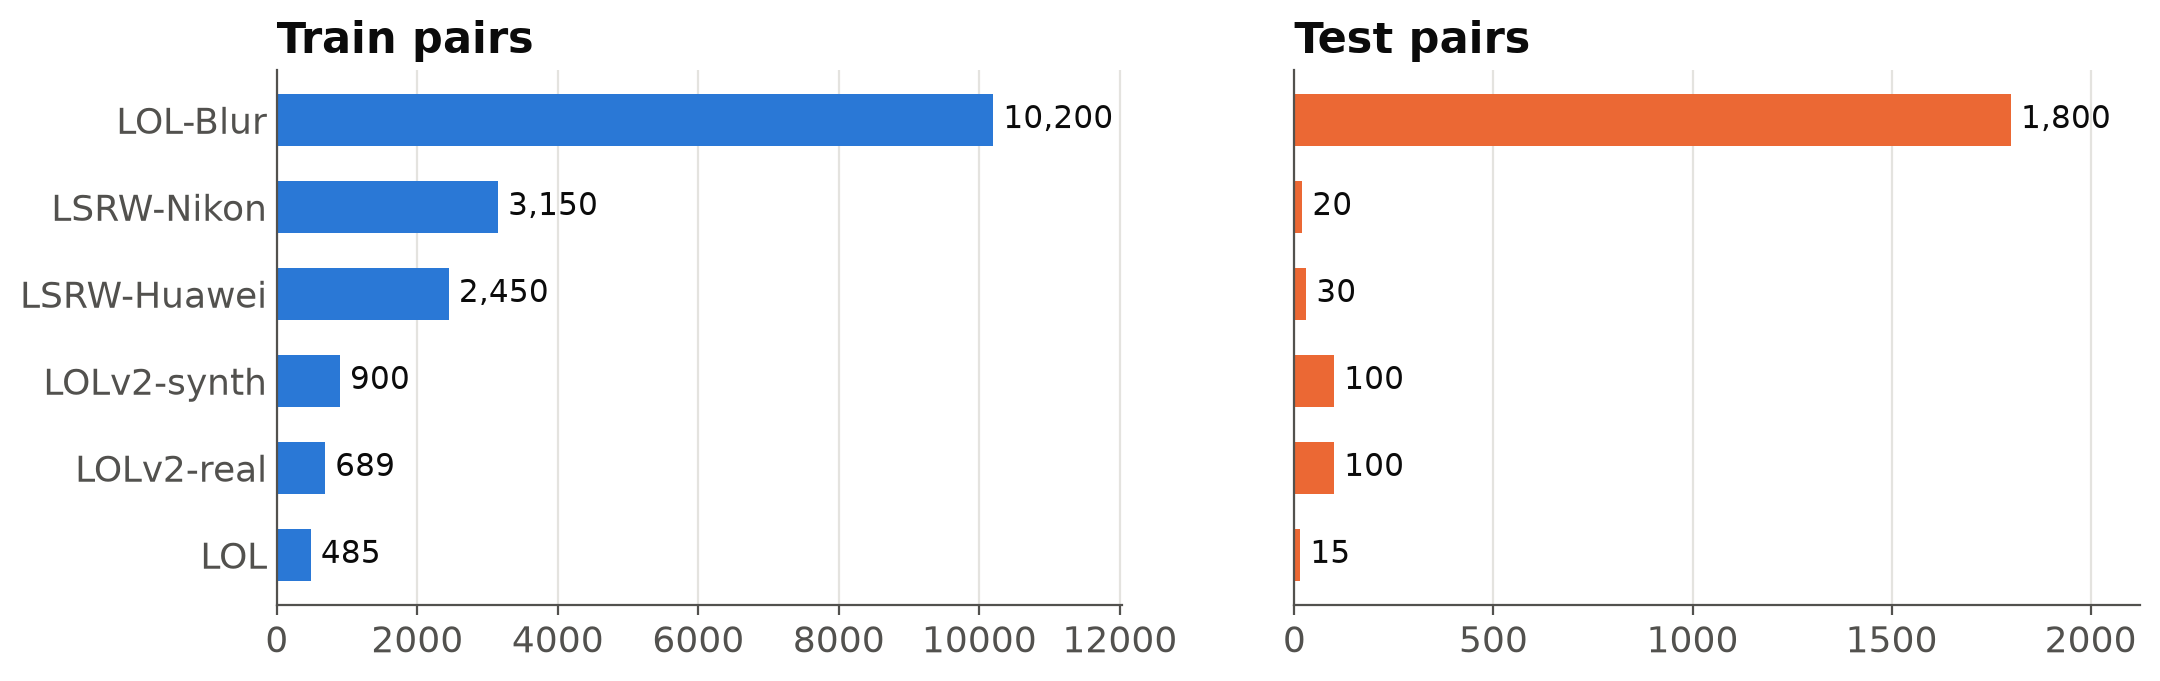
\includegraphics[width=0.95\textwidth]{eda/dataset_sizes.png}
%     \end{center}
%     {\footnotesize
%     \begin{itemize}
%         \item LOL-Blur alone has more training pairs than all other paired sets combined.
%         \item Test sets are tiny for LOL (15) and LSRW (20--30): single-number scores there are noisy.
%     \end{itemize}
%     }
% \end{frame}

% \begin{frame}
%     \frametitle{Backup: LOLv2 Samples}
%     \framesubtitle{Low-light input (top) vs.\ normal-light ground truth (bottom), test split}

%     \begin{center}
%         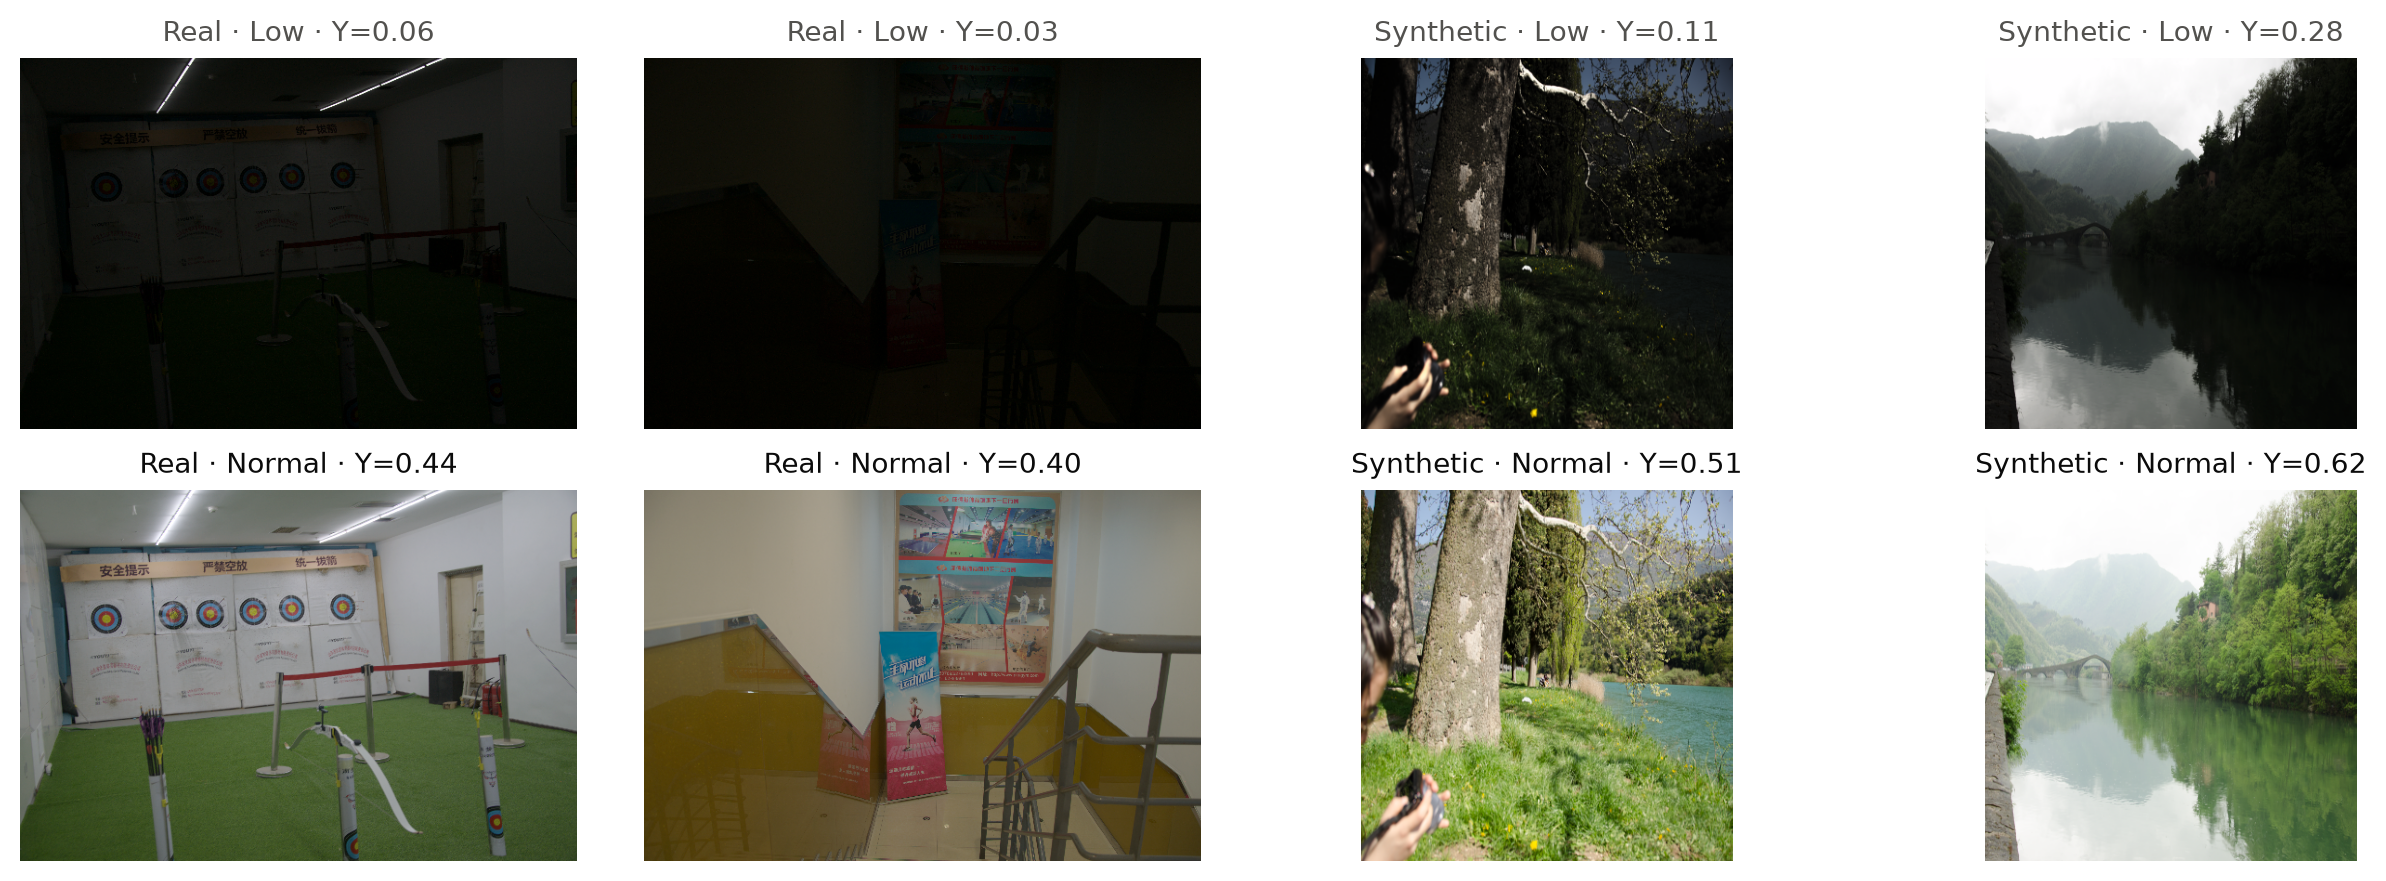
\includegraphics[width=\textwidth, height=0.6\textheight, keepaspectratio]{eda/samples.png}
%     \end{center}
%     {\footnotesize
%     \begin{itemize}
%         \item Real: 689 + 100 pairs, 600$\times$400. Synthetic: 900 + 100 pairs, 384$\times$384. All RGB, every low image has its ground truth.
%     \end{itemize}
%     }
% \end{frame}
% 12 - Closing slide
\begin{frame}
    \begin{center}
        
\includegraphics[height=1.5cm]{fptu_logo.png}\\[6mm]
        {\fontsize{40}{46}\selectfont\bfseries\color{fptBlue} Thank You!}\\[4mm]
    \end{center}
\end{frame}

\end{document}
